\begin{frame}{El PIB real de 2025 superó en 16,1\% el nivel de 2019}
\centering
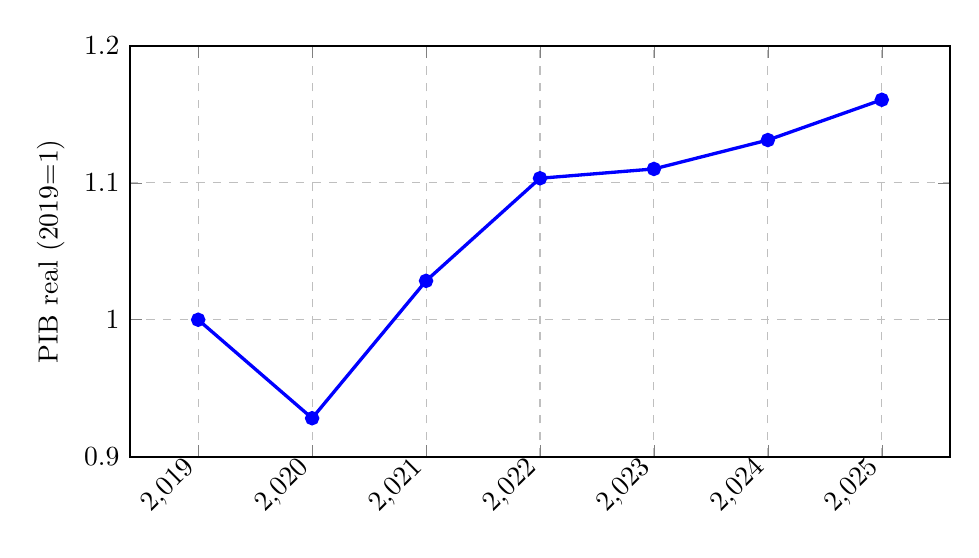
\begin{tikzpicture}
\begin{axis}[
    width=12cm,
    height=6.8cm,
    ylabel={PIB real (2019=1)},
    xtick={2019,2020,2021,2022,2023,2024,2025},
    xticklabel style={rotate=45,anchor=east},
    ymin=0.90,
    ymax=1.20,
    grid=both,
    grid style=dashed,
    thick
]
\addplot[color=blue,mark=*,very thick] coordinates {
    (2019,1.0000)
    (2020,0.9281)
    (2021,1.0284)
    (2022,1.1033)
    (2023,1.1101)
    (2024,1.1312)
    (2025,1.1606)
};
\end{axis}
\end{tikzpicture}
\vspace{0.15cm}
\scriptsize Fuente: DANE y MFMP 2026, tabla 1.2. Para 2025 se aplica el crecimiento real de 2,6\% reportado por el MFMP al nivel de 2024.
\note{[Sources] MFMP 2026, capítulo 1, tabla 1.2. Serie 2019-2024: DANE, como en la versión fuente.}
\end{frame}